% !TeX root = ../main.tex

\chapter{文獻回顧}

為彌合基於坐標之空間資訊與自然語言描述之間的鴻溝,本研究提出一個整合性框架,該框架結合位置語意、空間資料、空間操作與空間認知的理論基礎,旨在探討如何從圖徵所蘊含的位置語意,有效轉譯和理解自然語言中的位置描述。為建立研究基礎,本研究的文獻回顧將依循以下脈絡展開:

首先,探討語言學領域中關於位置描述的語言形式,以釐清本研究對位置描述之定義與範疇;其次,回顧文獻如何分析並建構地理空間的語意表達,特別關注位置描述的語言表徵、空間認知與空間資料三者的關聯,以作為本研究重要的理論基礎;第三,討論在語意形式化方法中,知識本體在語意建模和產生語言的潛在能力,說明本研究方法的核心概念;最後,整理目前語意式位置描述的研究發展,包含結構化紀錄與語意建模兩大途徑,並指出現有研究缺口與本研究預期的貢獻。

\section{位置描述的語言形式}

位置描述是自然語言中表徵空間資訊的方式,通常以目標物、空間關係與參考物構成的三元結構呈現,其語言形式受參考系統類型所影響。此結構近似於圖地理論(figure-ground theory),表示空間物件及其之間的空間關係,「圖(figure)」係為描述目標位置的目標物,而「地(ground)」則是參考物\citep{RN93, RN104}。例如,表達一坐標值時,是基於目標物與地理坐標系之間的關係。同樣地,即便如地名的表達上雖未明示空間關係,仍然隱含相等或包含等空間關係。例如,「台北」與「台北市」具有清晰語意的地名具有可識別性,可省略空間關係詞直接作為位置描述\citep{RN93}。

\citet{RN2}從語言形式的視角提出了三種參考系統類型:相對(relative)、絕對(absolute)與內在(intrinsic),構成了位置描述的基本語言架構,不僅反映人類的空間認知方式,也為語言處理與空間資訊系統中的位置理解與運算提供了關鍵理論基礎。在相對參考系統中,位置描述依觀察者的視角而定,例如「圖書館的左側」是基於觀測者視角下認定圖書館與目標物的關係而決定;絕對參考系統則基於物理環境的固有屬性來描述空間關係,例如「台北市東南邊」是基於八方位的方位系統而定,對於不同位置上的觀測者而言,都能夠從位置描述中正確辨識位置。至於內在參考系統,其描述方式依賴參考物的語意屬性,例如「台北101前面」是基於建築物本身的方向性而定義。

除了參考系統與三元結構的分析外,語言學領域也廣泛探討構成位置描述的詞彙組成,常見有空間介詞與方位詞的討論。介詞(preposition)可定義為「 a function word that typically combines with a noun phrase to form a phrase which usually expresses a modification or predication」\citep{RN188},可譯為通常與名詞片語結合形成片語,並用於表示修飾或述語的功能詞。專指空間概念的介詞常被稱為「空間介詞(spatial prepositions)」,如英文中的「in(在…裡面)」與「behind(在…後面)」等。在中文語境中,位置描述的空間關係部分同時依賴介詞和「方位詞」為共同組成單元,例如「在…裡面」中,「在」為空間介詞,「裡面」為方位詞\citep{RN46, RN189, RN190}。方位詞具備指示方向與位置的功能,常見例子包含「上/下」、「前/後」和「東/西/南/北」等,並常搭配介詞使用以構成完整的空間語句。


\section{地理空間的語意}

地理空間(Geographic space)的語意不僅涵蓋其物理結構與資料層級,更深層地反映了人類如何透過認知框架理解並表達地理空間與現象,在GIS過往研究中主要探討如何處理空間資料背後的語意,以建構對地理現象的理解與描述模式,相關研究大致可分為兩類取徑。其一類研究著重探討人如何理解地理空間的結構性框架。\citet{RN25}認為應用知識本體於地理環境中,可表示了地理上的物理空間,可以概念化人類如何去理解「地理空間」。\citet{RN43}進一步提出一個「空間概念」、「空間物件」和「幾何符號」三者相互關聯的架構,藉此整合異質的地理資料來源,提升語意一致性與資料可交換性。

另一類研究則關注地理現象的知識建構,\citet{RN161}提出了「地理情境(geographic scenarios)」與「地理特徵(geo-characterization)」兩個核心概念,,以捕捉地理現象在具體脈絡中的語意結構。「地理情境」由位置、時間、事情、人、活動及現象六個結構組成,而這些維度又可進一步細分,以具體描述情境中地理現象的細節。「地理特徵」則用來描述地理情境之關係。該概念模型透過「地理情境」、「基於實體的要素」和「時空要素」達成捕捉地理空間與現象。舉例而言,輸入一個城市,可以知道它隸屬於什麼行政區、包含哪些子行政區、擁有多少人口和國內生產毛額(gross domestic product, GDP)等資訊。當中地理情境是指該城市,基於實體的要素是指行政區劃且有著明確空間範圍該城市,而時空要素說明了它的人口、GDP等。

此外,在人文地理學研究中,人與地理空間的互動常常以「地方(place)」作為核心概念,並涉及與空間認知相關的三個層次:物理空間(physical space)、認知空間(cognition space)及表徵空間(representational space)。其中,物理空間係指人們所處的客觀環境;認知空間則是人對於空間的理解與主觀感受;表徵空間則是透過語言、圖像、圖徵或符號所建構出的外顯形式。過去不同學者已從該角度提出不同名詞和定義的模型,\citet{RN131}認為地方的意義是透過自我、他人和環境三者構建的,顯示人與地理空間互動存在感知的過程;\citet{RN57}認提出人透過物理、邏輯、表徵及認知四個「universe」來感知地理空間。

更進一步地,\citet{RN128}引入了「空間認知(spatial cognition)」的理論,劃分「真實空間」、「描述空間」及「認知空間」三個層次,闡明人類如何從所感知的真實空間,透過認知與語言表徵的過程,形成具備語意的位置描述。這一框架指出,當人類接受到一個位置描述的請求時,會透過其過往經歷的真實空間重建空間概念,並調用認知空間中的概念表徵,最終透過語言進行位置語意的表達。認知空間在此扮演中介角色,其來源為感知經驗的內化,而語言則將此內化知識外顯化為具體描述。

因此,本研究亦借鏡\citet{RN128}提出基於空間認知的觀點產生位置描述,試圖建構人類產生位置描述的過程模型(參見\ref{fig:congition})。藉由探討人在接收位置詢問時,如何從其認知空間中對空間物件的概念,並結合語言系統進行概念化與語意表達,進一步揭示語言中位置描述的生成機制。此一過程不僅涉及物理空間的感知經驗,也反映出語言、概念與空間之間的深層連結。

\begin{figure}[!htbp]
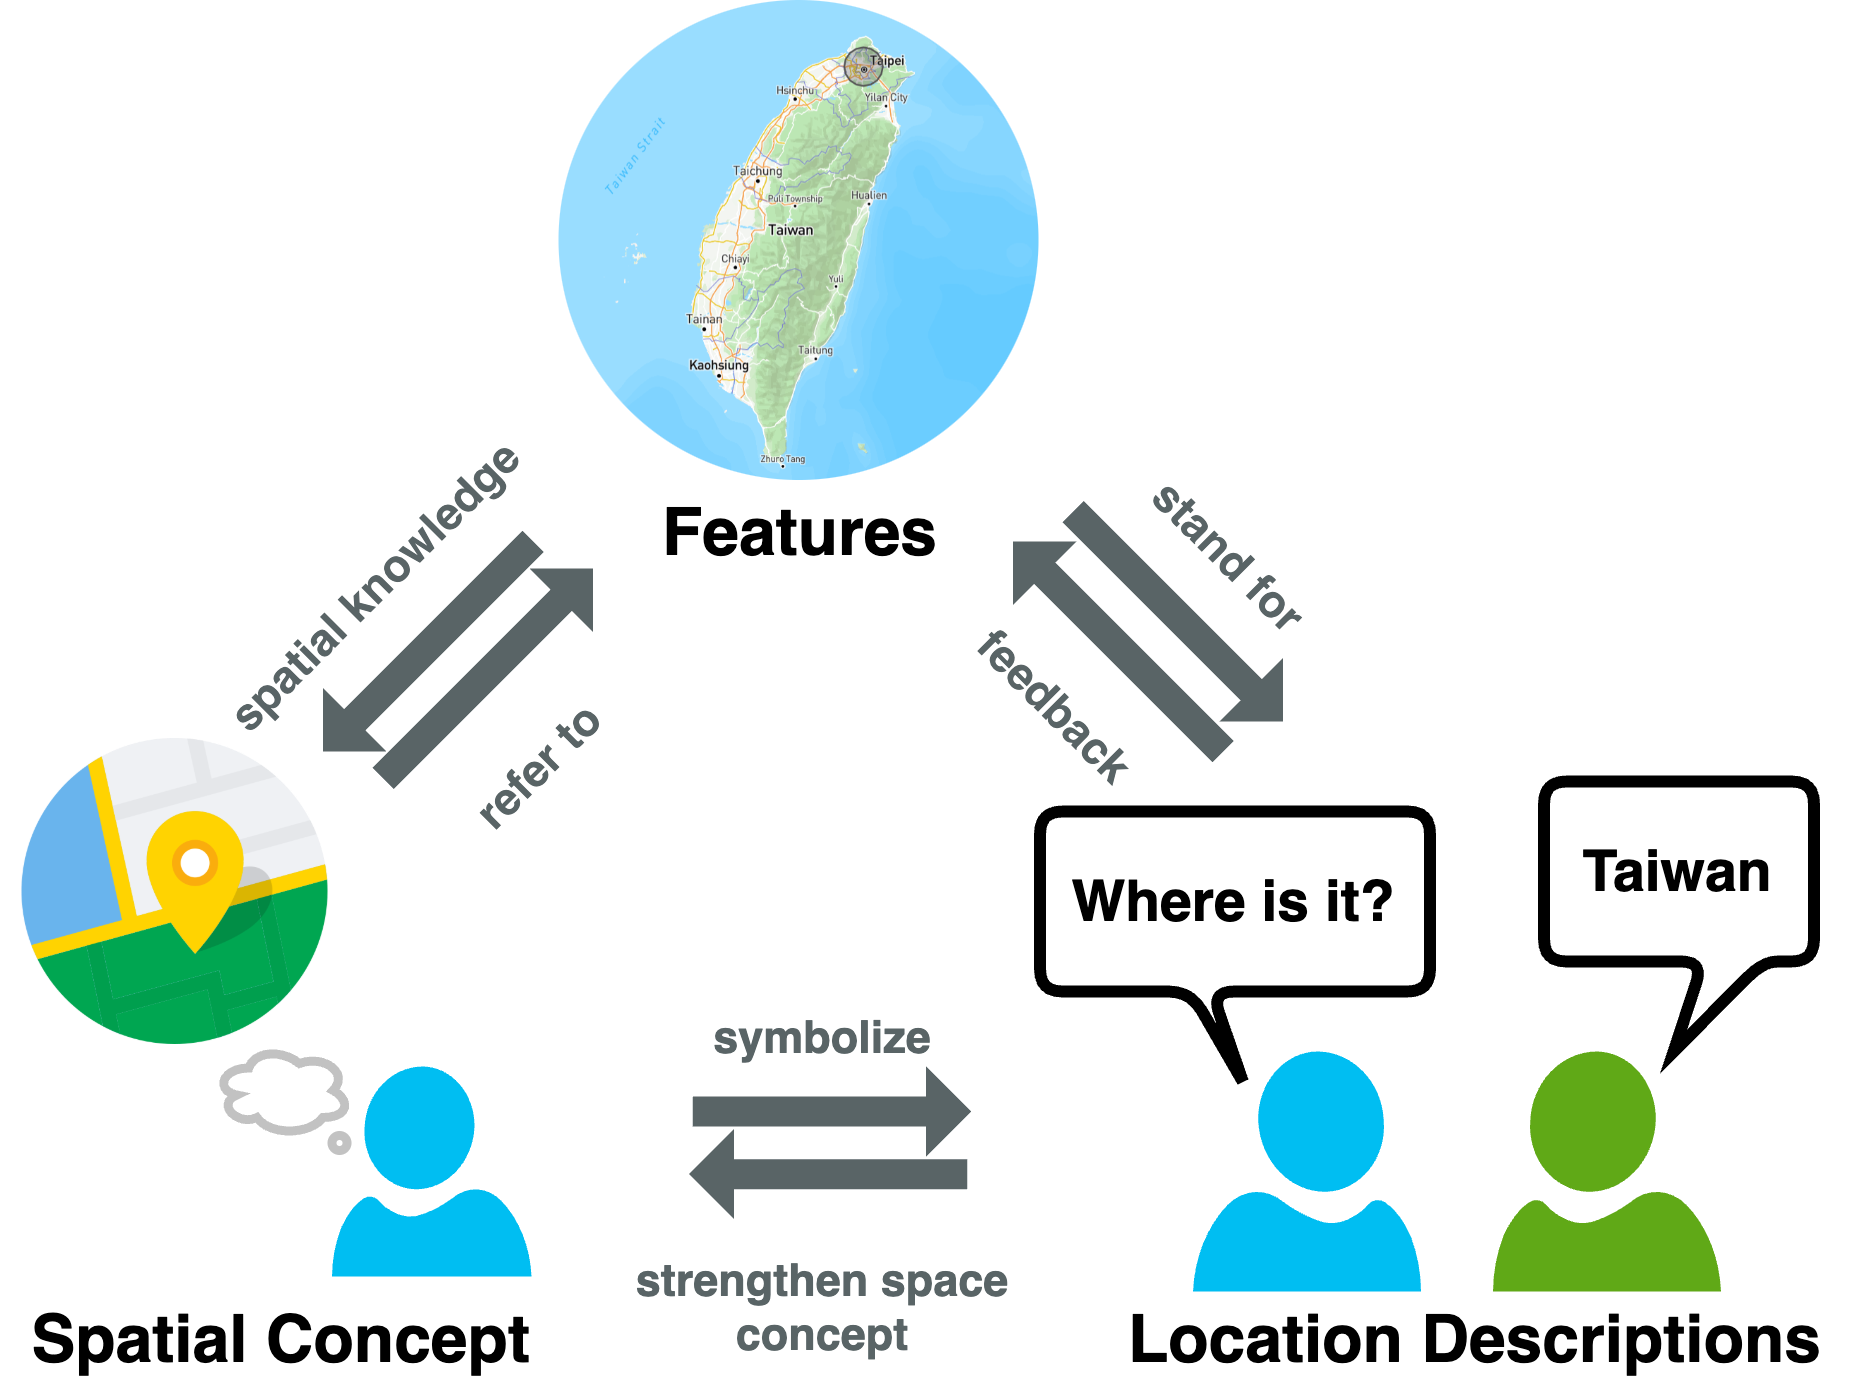
\includegraphics[width = \textwidth]{figures/congition.png}
\centering
\caption{位置描述語意三角形(改自\citet{RN128})}
\label{fig:congition}
\end{figure}

\section{知識本體與產生自然語言}

知識本體是一個形式化語言模型,具有以下三個核心要素:概念(concept)或類別(class)、實例(individual)與關係(relation),用以表示特定領域中物件的類型、結構、屬性、過程和關係\citep{RN24} 。地理現象可藉由知識本體形式化,舉例而言,行政區劃的空間關係「台北市包含大安區」這一現象,可以透過知識本體形式化為類別「County(縣市)」與「District(區)」,與之對應的實例為「台北市」與「大安區」,關係則可以表示為「hasContain(包含)」,即「台北市」作為一個實例,與「大安區」透過hasContain關係相連。這一語意結構的建模能力,使知識本體得以有效捕捉日常生活中的空間知識,並提供作為語意層次查詢與推理,例如,在該例中欲查詢行政區所包含的物件,即可獲得「大安區」的內容。

基於知識本體的語意建模能力,知識本體不僅可用於資料整合與邏輯推論,也逐漸被應用於產生自然語言的研究中。透過類別、實例與關係的結構化表示,可支持語言描述中角色、事件與語意關係的抽象建模,進而實現產生基於語意的文字。在非空間領域中,\citet{RN163}將知識本體應用在電子健康檔案上,將結構化紀錄的健康資訊轉換為自然語言文字,以協助醫療人員的解讀。在地理資訊領域中,經常以具備語意特徵的屬性資料作為地圖輔助描述\citep{RN165, RN166}。這類研究根據提出文檔計畫(document planning)過程中事先擬定好相關的參數及文字描述,使地理資料得以以自然語言描述方式呈現。惟這類研究多著重於地圖可視化中變量的敘述,如地形、設施數量等,較少涉及位置本身的語意建構與推論生成機制。

\section{知識本體與產生自然語言}

為了解決自然語言位置描述中所蘊含的語意模糊性與語境依賴性的挑戰,過往研究逐漸將語意層面納入從基於坐標之空間資料產生位置描述或逆向地理編碼中。此類研究大致可分為三類方法:依賴結構化地名資料(如地名辭典(gazetteers)和知識圖譜)和使用模糊邏輯與語意模型進行位置表示。

首先,地名辭典(gazetteers)作為逆向地理編碼的基礎資料來源之一,扮演結構化空間語意的角色,其常以地名、地點類型及其對應的空間足跡(spatial footprints)為三種基本構成元素\citep{RN122, RN159, RN31},試圖將語言中的地名對應到具體空間範圍及地理空間實體。近年來,為期獲得接近人類對於實體世界的表達,運用社群媒體資料建構更具有語意細緻度的地名辭典,藉此貼近人類對實體世界的描述習慣\citep{RN31}。相對於地名辭典的紀錄,\citet{RN23}則一樣透過社群媒體資料,但以地方圖譜(place graph)儲存人對實體世界的表達。該圖譜由空間物件及空間關係組成,因而產生合適地名不需要依賴傳統GIS空間分析方法,而是依照知識圖譜中記錄下自然語言式的空間關係三元組。儘管這些資料和儲存格式有助於提升逆向地理編碼產生位置描述的準確度和豐富度,結構化格式難以完整和全面涵蓋語言中隱含的模糊性與相對位置描述,在語意處理能力上仍具限制。

為克服此限制,研究開始探索以模糊邏輯與語意模型的方式來處理基於坐標之空間資料與位置描述的連結。例如,\citet{RN133}透過社群媒體資料計算隸屬函數(membership function)分析人類對「南/北加州」的認知,建立隸屬函數網格推估具有模糊邊界的地名空間範圍,有效捕捉地名的認知模糊性;\citet{RN164}針對相片地點的自然語言產生,提出一組顯著性指標(如照片地點是否常出現、地名的稀少和重要性、距離等),挑選適切之參考地名,再判斷其與目標坐標間的空間關係,並加上空間介詞來形成位置描述的方式。該研究針對地名產生僅能達到相對位置的描述,然而缺少在日常生活中也常使用到的絕對位置描述;而在\citet{RN128}的研究中,深入的討論了位置描述語意模糊性的原因,並以超值理論(supervaluation)為存在模糊的位置描述提出了一個定量的框架及機制,並透過問答系統使得研究貢獻得以應用於GIS上。該研究指出參考系統、空間物件(spatial object)和空間關係(spatial relationship)三者是造成模糊性的原因,首先,描述的參考系統影響了人類如何辨識空間物件及認知空間,存在於不同觀測者的空間認知和能力中,因此難以直接從描述中獲取。其次,空間物件可再細分為參考物與目標物件,不同觀測者間於認知中辨識出的物件也會有不同,除了物件的名稱外,物件的屬性資料也可能被用來進行描述,例如:大小和高度。最後,空間關係,例如「near」一詞根據不同觀測者會有其對應的定量值。該研究於過往對於空間認知的文獻設定變數改變其權重,以達成透過定性資料處理定量的地理資訊,並能提供都市導航的指路選擇。

整體而言,這些研究指出僅依賴坐標或結構化的地名資料儲存進行逆向地理編碼或語意查詢時,難以全面捕捉自然語言位置描述中蘊含的語意模糊性、情境依賴性與認知差異性。雖然透過給定語意建模或模糊邏輯等手段,有助於提升處理部分語意不確定性,卻仍缺乏一套能整合「位置描述詞彙、空間資料、語意空間關係、認知視角」的通用形式化表示與推理機制。此外,目前相關方法多偏重於語意輸出,但對於如何系統性建模空間語意概念之間的結構性關係,例如參考物、目標物與空間關係之間的角色與制約關係,尚缺乏深入處理。因此,本研究欲填補此一缺口,嘗試引入知識本體的形式化能力,結合語意規則推理,整合空間資料、語言表徵與空間認知概念,建構一套可推論之語意式位置描述的框架,進一步提升自然語言與空間資訊之間的語意連結與轉譯能力。

